\section{Test-bed Environment and Experiments}
\label{sec:evaluation}

This section will explain and show how this project was tested while implemented as shown in Section \ref{sec:implementation}. There was lots of trial and error scenarios and all testing was performed before fully implementing a technology stack, by manually trying if the technology implementation was working as intended to.

Therefore the main method of testing in this project was, manually testing with trial and error without any premade testing software's or methods.
\subsection{Data Access Object testing}
As mentioned in Section~\ref{sub:jpa}, the first things implemented were USER and POLL entities. So testing their implementation and relations between them, was the beginning of any testing. To perform tests on entities, entity DAO's were used with some simple CRUD operations; create a user and poll, edit created user and poll, delete created poll and user, and read information of created poll and user.

\subsection{REST API testing}
Further implementation and development of this project consisted of going from DAO classes to Spring JPA implementation and adding some control over these entities from "outside" of the code, a REST API. This meant a different approach to testing of the implementation. Now some simple code wasn't sufficient enough, thus a software that could send HTTP requests to the project application, which then acted accordingly to the requests was required. For this testing method, Postman \cite{postman} was used.
\subsubsection{Postman}
Postman is an Open-Source software that can send user defined requests, consisting of JSON body or include path variables to customize requests for own preference. These requests can be of any type (GET, POST, PUT, DELETE, ...). After sending a request from Postman, it will receive the response according to sent requested. Response will also include HTTP status code for success or error, this was very helpful for testing and to see if implementation of REST API was correctly assembled. This made all testing very simple and the error backtracking was easier. Postman was the main method of testing all client (user) interactions with the program, until security and model view was implemented.

\begin{figure}[H]
  \centering
  \begin{minipage}{0.4\textwidth}
    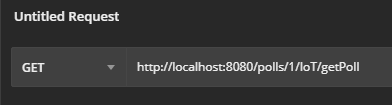
\includegraphics[width=\textwidth]{figs/postmanrequest.png}
    \caption{Postman request.}
    \label{fig:postmanrequest}
  \end{minipage}
  \hfill
  \begin{minipage}{0.4\textwidth}
    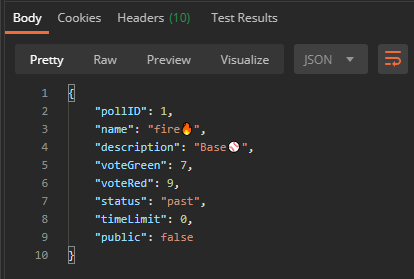
\includegraphics[width=\textwidth]{figs/postmanresponse.png}
    \caption{Postman response.}
    \label{fig:postmanresponse}
  \end{minipage}
\end{figure}

\subsubsection{HTML/CSS}
After implementing Security, an authorization token was required to use most services. So the only way to test, was to manually go on the web page and see if the service implemented was working properly and as intended or if something could be done differently. Authentication security was therefore turned on after client interaction with FeedApp was behaving as mentioned in prototype design application flow Section~\ref{sub:appflow}.

This method of testing was also used when the CSS was added to the project web application and with CSS, the testing was made more "user friendly". Even though testing was performed on Postman and via the features distributed from it. The whole project after fully developed, does not use or have features available to receive request based on JSON body, such that Postman requests can be performed. All HTML and CSS implementation was based on own education and own preferences, to how things would optimally work and look, but also easy to understand for the client when using the service. When errors occurred during CSS development, some basic tutorials were looked up on w3schools \cite{w3css} and errors resolved quickly after.

\subsubsection{IoT testing}
IoT used for this project was a simple Java program as mentioned in Section~\ref{subsub:IoTsupport}. So testing if the implementation was working correctly and error-less, was a tedious process to manually check all possible user input errors. Many tests required many restarts of the Java program, but also many look-ups on the web page. Web page user interaction was already implemented, so the testing was possible to perform without sending request and getting responses through Postman. Therefore also possible to save time and amount of required clicks.